\documentclass{beamer}
\usepackage[utf8]{inputenc}
\usepackage{graphicx} % For including images

% Theme (optional, choose one you like)
\usetheme{metropolis} % Example theme

\title{Holographic Interferometry}
\subtitle{Photonics Final Presentation}
\author{Andreu Snijders} % Replace with your name
\date{\today}

\begin{document}

\frame{\titlepage}

\section{Introduction}
\begin{frame}{What is it holographic interferometry?}
    Holographic interferometry is a powerful optical technique that combines the principles of interferometry and holography.
    \begin{itemize}
        \item \textbf{Interferometry:} A family of techniques in which waves, usually electromagnetic waves, are superimposed, causing the phenomenon of interference in order to extract information.
        \item \textbf{Holography:} The science and practice of making holograms, which are three-dimensional recordings of a light field.
    \end{itemize}
    This presentation will explore the fundamental concepts behind holographic interferometry and its diverse applications.
\end{frame}

\section{Interferometry}
\begin{frame}{Interferometry: The Basics}
    To understand holographic interferometry we should first be familiar with the basic principles of interferometry:
    \begin{itemize}
        \item Wave superposition
        \item Coherence requirements
        \item Types of interferometers (e.g., Michelson, Mach-Zehnder)
        \item Applications in metrology
    \end{itemize}
\end{frame}
\begin{frame}{Interferometry: Wave superposition}
    When two or more waves overlap in space, the resulting wave amplitude is the algebraic sum of the individual wave amplitudes.
    
    \vspace{0.5em}
    
    For two coherent light waves with amplitudes $E_1$ and $E_2$:
    \begin{equation}
        E_{total} = E_1 + E_2 = A_1 e^{i(\omega t + \phi_1)} + A_2 e^{i(\omega t + \phi_2)}
    \end{equation}
    
    \begin{itemize}
        \item \textbf{Constructive interference:} When waves are in phase ($\Delta\phi = 0, 2\pi, 4\pi...$)
        \item \textbf{Destructive interference:} When waves are out of phase ($\Delta\phi = \pi, 3\pi, 5\pi...$)
        \item \textbf{Intensity:} $I \propto |E_{total}|^2 = I_1 + I_2 + 2\sqrt{I_1 I_2}\cos(\Delta\phi)$
    \end{itemize}
\end{frame}
\begin{frame}{Interferometry: Wave superposition}
    \vspace{0.4cm}
    \begin{figure}[h]
        \centering
        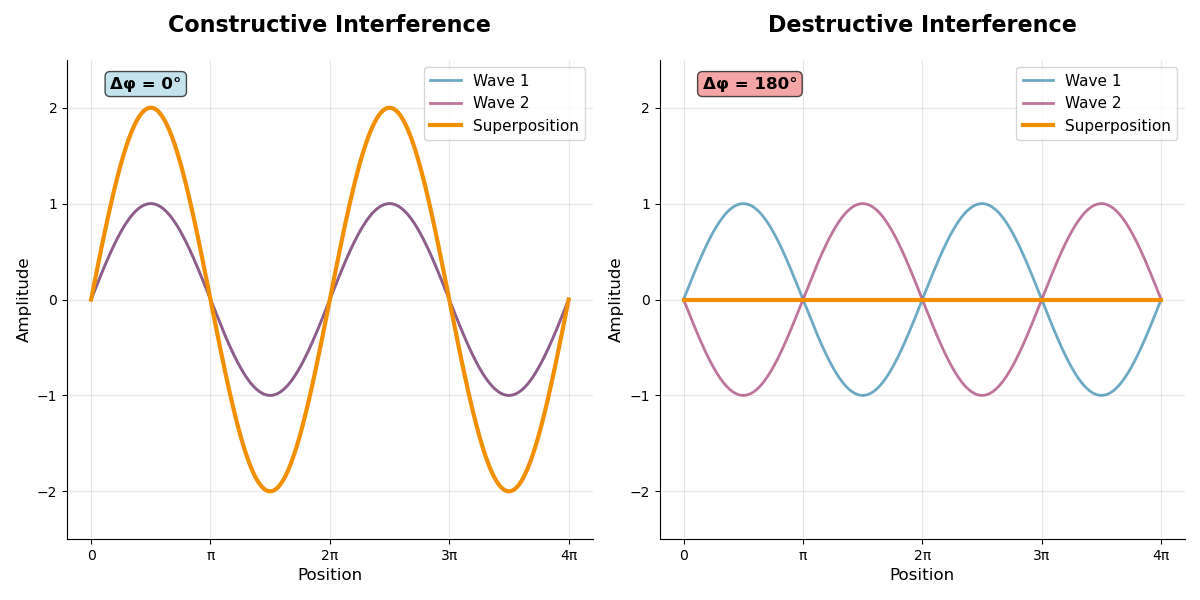
\includegraphics[width=1\textwidth]{Figures/constructive-destructive-interferences.png}
        \caption{Illustration of wave superposition showing constructive interference (left) where waves add in phase to create larger amplitude, and destructive interference (right) where out-of-phase waves cancel each other.}
        \label{fig:interference}
    \end{figure}
\end{frame}
\begin{frame}{Interferometry: Coherence requirements}
    For stable interference patterns, light sources must exhibit:
    
    \begin{block}{Temporal Coherence}
        \begin{itemize}
            \item Light must be \textbf{monochromatic} (single frequency/wavelength)
            \item Coherence length: $L_c = \frac{\lambda^2}{\Delta\lambda}$
            \item Path difference must be $< L_c$ for visible fringes
        \end{itemize}
    \end{block}
    
    \begin{block}{Spatial Coherence}
        \begin{itemize}
            \item Light source must be sufficiently \textbf{small} or \textbf{collimated}
            \item Ensures constant phase relationship across the wavefront
            \item Critical for uniform fringe visibility
        \end{itemize}
    \end{block}
    
    \vspace{1em}

    \hrule
    
    \begin{alertblock}{Practical Sources}
        \textbf{Lasers} are ideal: high temporal and spatial coherence \\
        \textbf{LEDs/lamps} require filtering and careful design
    \end{alertblock}
\end{frame}
\begin{frame}{Interferometry: Coherence requirements}
    
    \begin{figure}[h]
        \centering
        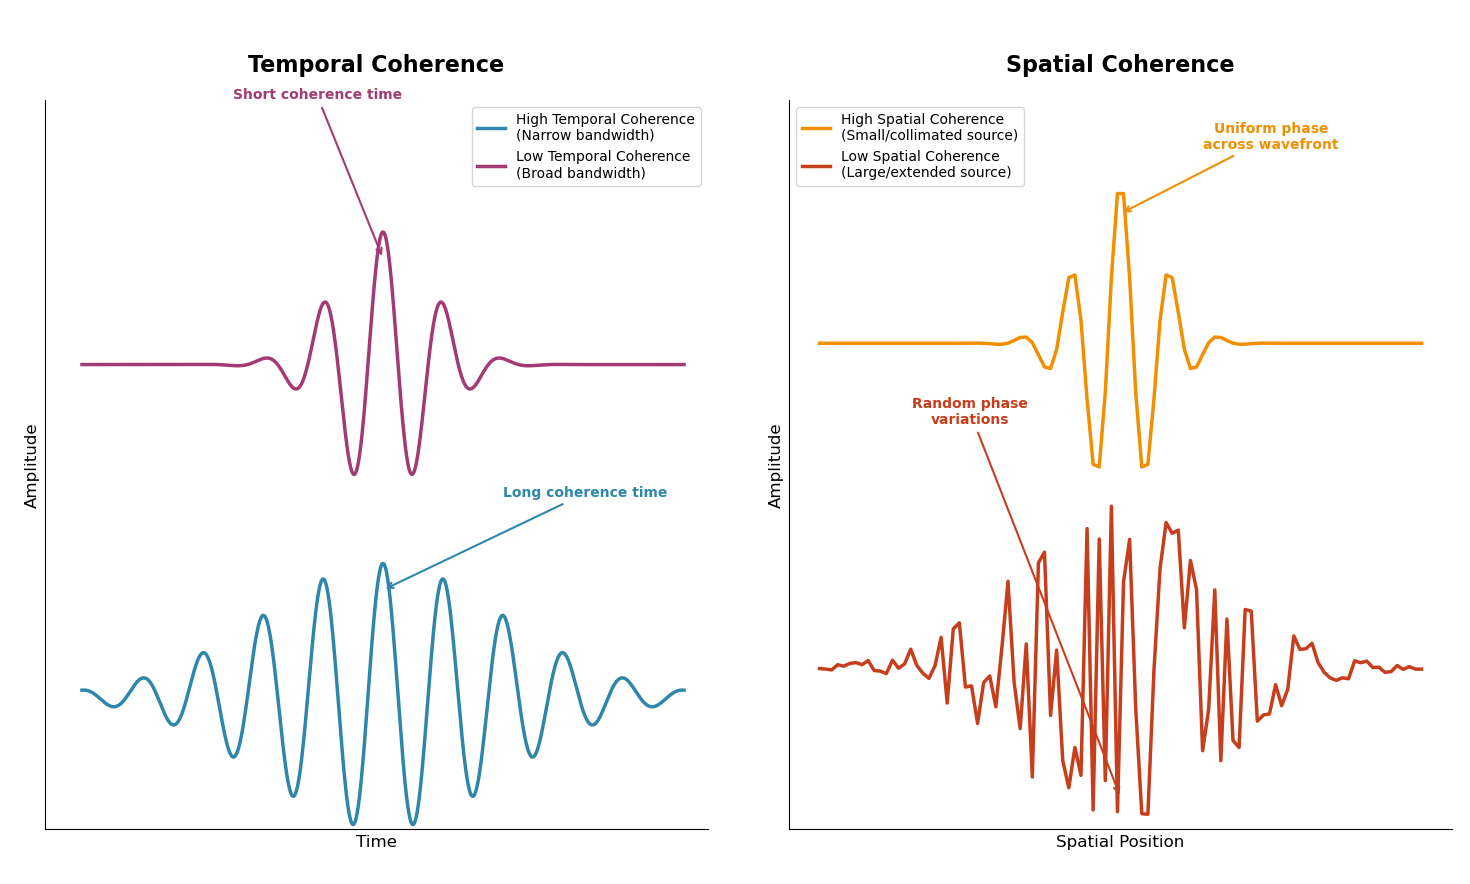
\includegraphics[width=0.87\textwidth]{Figures/temporal-spatial-coherence.png}
        \caption{Demonstration of coherence requirements: temporal coherence (left) shows the need for monochromatic light with sufficient coherence length, while spatial coherence (right) illustrates the importance of wavefront uniformity for stable interference patterns.}
        \label{fig:coherence}
    \end{figure}
\end{frame}
\begin{frame}{Interferometry: Types of interferometers}
    \vspace{0.2cm}
    \begin{figure}[h]
        \centering
        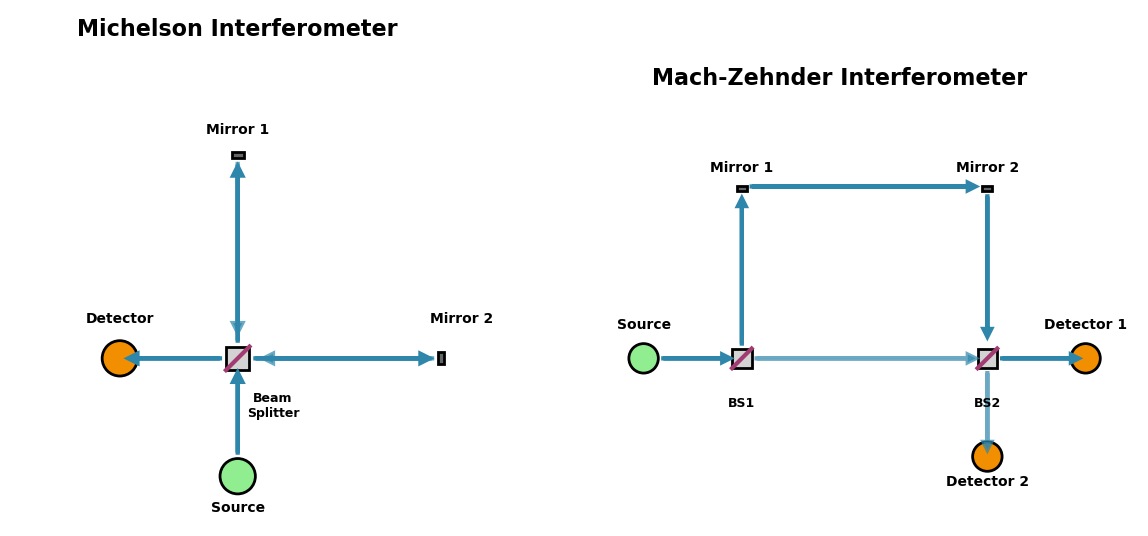
\includegraphics[width=0.9\textwidth]{Figures/interferometers-types.png}
        \caption{\textbf{Left:} Michelson interferometer - measures length changes by detecting phase shifts in interference fringes when one mirror moves, enabling nanometer-scale displacement detection. \textbf{Right:} Mach-Zehnder interferometer - compares optical path lengths between two separate beams, allowing measurement of refractive index changes, object thickness, or phase disturbances in one arm.}
        \label{fig:interferometers}
    \end{figure}
\end{frame}
\begin{frame}{Interferometry: Applications in metrology}
    \begin{itemize}
        \item \textbf{Length and distance measurement}  \\
        \quad Interference fringes shift as the optical path length changes \\  
        \quad ($nm$ resolution or higher)
        \vspace{0.3em}
        \item \textbf{Surface profiling and surface} \\ 
        \quad Comparing an optical surface to a reference flat or spherical \\
        \quad surface to reveal deviations, roughness... \\ 
        \quad (again, $nm$ resolution or higher)
        \vspace{0.3em}
        \item \textbf{Refractive index measurements} (precise phase shift \\
        \quad detection)
        \vspace{0.3em}
        \item \textbf{Wavefront Sensing} \\
        \quad Comparing the phase of a light wave emerging from an \\
        \quad optical system to that of a reference wave reveals wavefront \\
        \quad distortions caused by imperfect mirrors or lenses. 
    \end{itemize}
\end{frame}

\section{Holography}
\begin{frame}{Holography: Recording 3D Information}
    In order to fully  understand holographic interferometry we should also revisit some key aspects of holography:
    \begin{itemize}
        \item Recording process (interference and diffraction)
        \item Reconstruction process
        \item Types of holograms (e.g., transmission, reflection)
        \item Key differences from traditional photography
    \end{itemize}
\end{frame}
\begin{frame}{Holography: Recording process}
As explained, interferometry can be used to measure lengths and distances with high precision. If we measure planes (images) instead of single points we can create surface details and create 3D scans.
\end{frame}
\begin{frame}{Holography: Recording process}

\textbf{Our simulation (conceptual):}
\begin{itemize}
    \item Shows how distance variations create interference patterns
    \item Projects 3D surface information into 2D views
    \item Demonstrates the \textit{principle} of encoding 3D information in fringes
\end{itemize}

\vspace{0.3em}

\textbf{Real holography:} Object beam (scattered from object) + Reference beam interfere on a \textit{recording medium} (photographic plate/CCD). Our simulation is \textbf{educational} - it shows the concept but simplifies the actual recording process.

\vspace{0.3em}

The complex fringe patterns demonstrate how 3D surface variations get encoded.
\end{frame}
\begin{frame}{Holography: Recording process}

\textbf{Where are the light sources?}
\begin{itemize}
    \item \textbf{Front measurement:} Light source at position [0, 0, 3] - illuminating from +Z direction
    \item \textbf{Side measurement:} Light source at position [3, 0, 0] - illuminating from +X direction  
    \item \textbf{Top measurement:} Light source at position [0, 3, 0] - illuminating from +Y direction
\end{itemize}

\vspace{0.5em}

Each position acts as both:
\begin{itemize}
    \item \textbf{Light source} (object beam origin)
    \item \textbf{Reference point} for distance measurements
\end{itemize}

\vspace{0.3em}

Distance from source to each surface point determines the interference pattern recorded from that viewing angle.
\end{frame}
\begin{frame}{Holography: Recording process}
    \begin{figure}[h]
        \centering
        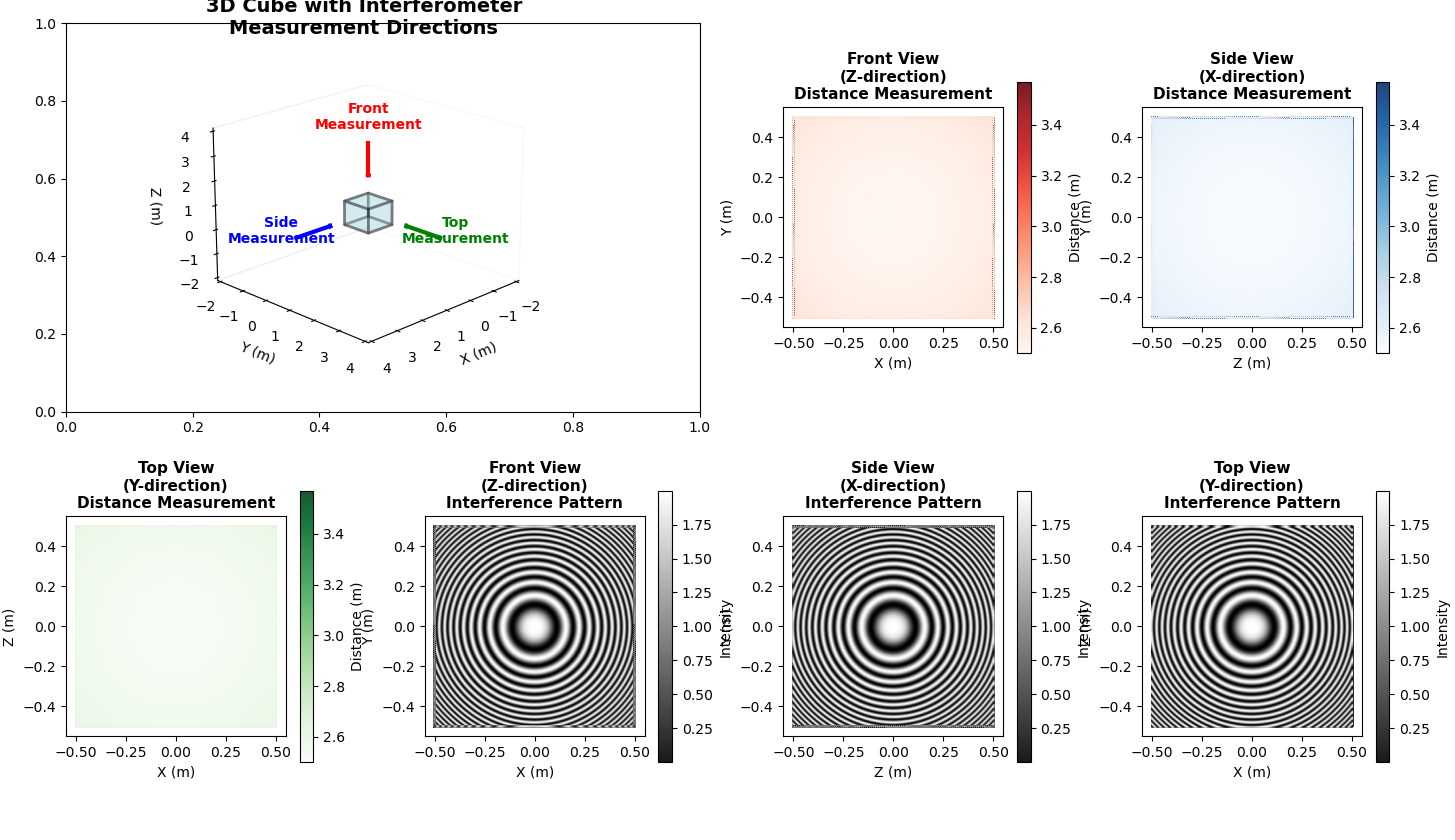
\includegraphics[width=1\textwidth]{Figures/cube-holograph.png}
        \caption{Interference patterns on flat surfaces of a 3D modelled cube.}
        \label{fig:cube_holograph}
    \end{figure}
\end{frame}
\begin{frame}{Holography: Recording process}
    \begin{figure}[h]
        \centering
        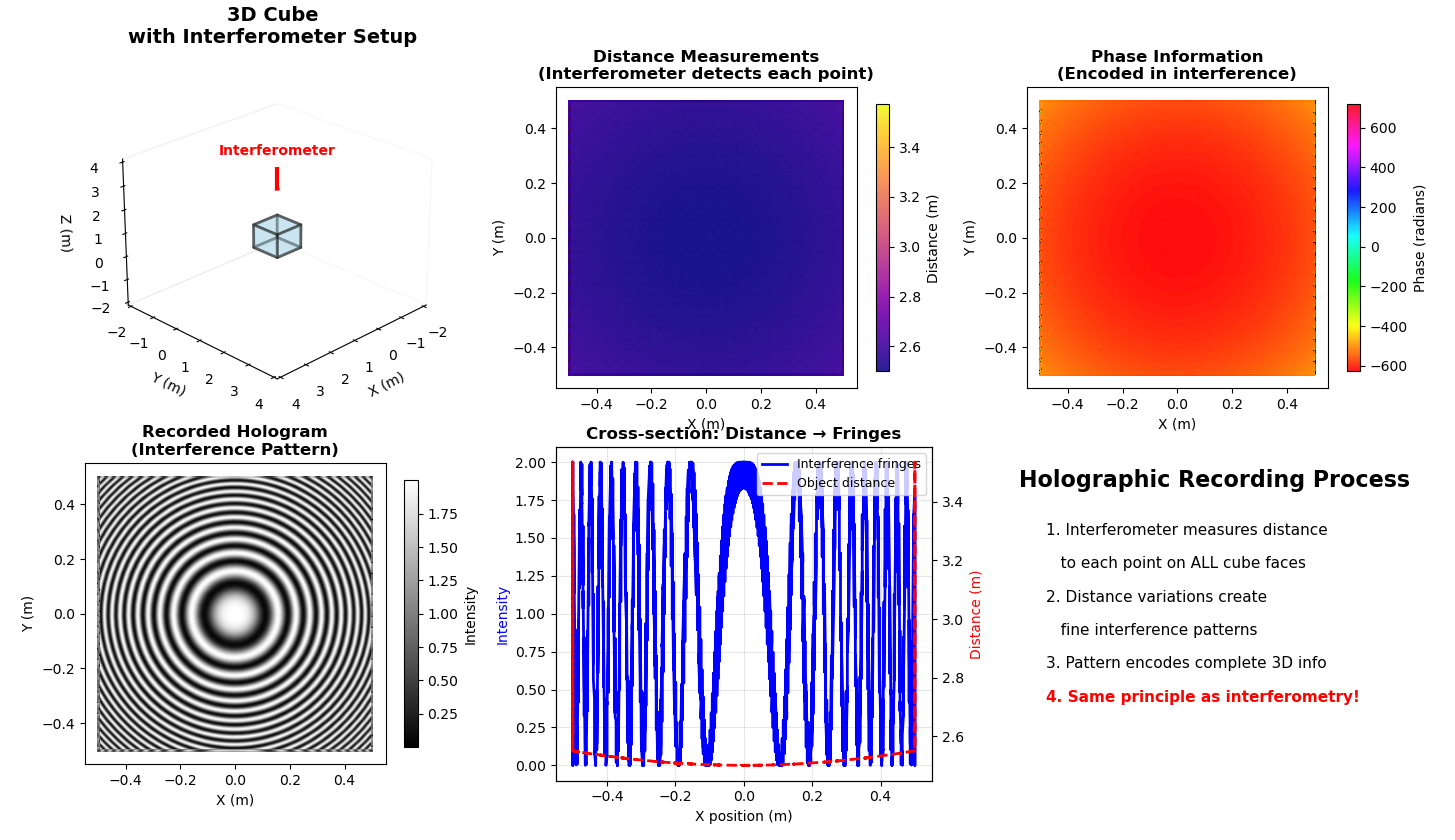
\includegraphics[width=1\textwidth]{Figures/cube-fringe-distances.png}
        \caption{Difference between fringes and the equivalent distance measurement values on a 3D modelled cube.}
        \label{fig:cube_fringes}
    \end{figure}
\end{frame}
\begin{frame}{Holography: Recording process}
    \begin{figure}[h]
        \centering
        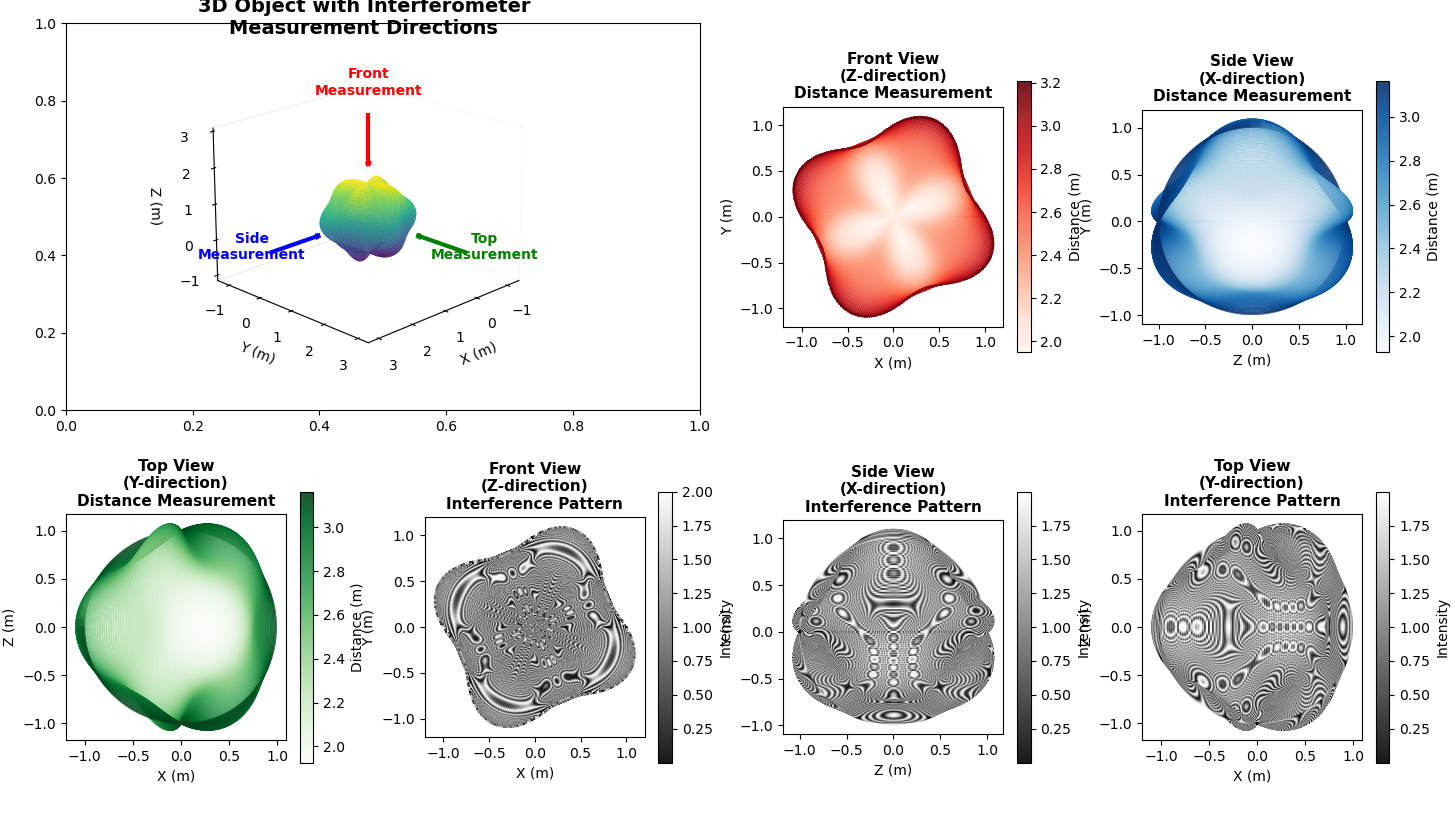
\includegraphics[width=1\textwidth]{Figures/sphere-holograph.png}
        \caption{Interference patterns on flat surfaces of a 3D modelled complex volume.}
        \label{fig:sphere_holograph}
    \end{figure}
\end{frame}
\begin{frame}{Holography: Recording process}
    \begin{figure}[h]
        \centering
        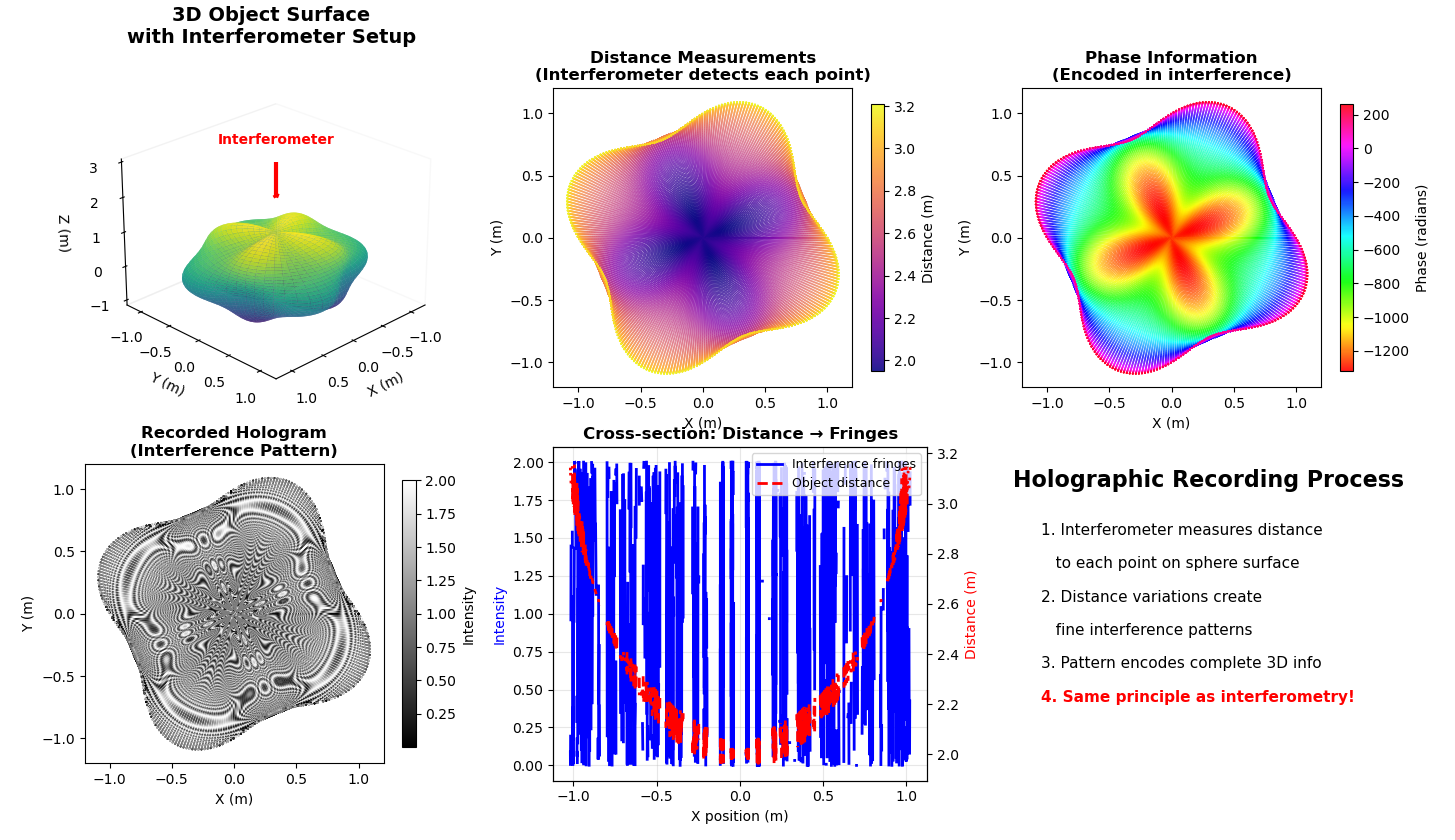
\includegraphics[width=1\textwidth]{Figures/sphere-fringe-distances.png}
        \caption{Difference between fringes and the equivalent distance measurement values on a 3D modelled complex volume.}
        \label{fig:sphere_fringes}
    \end{figure}
\end{frame}
\begin{frame}{Holography: Reconstruction process}
    To view the 3D information stored in the hologram, we reverse the recording process:
    
    \vspace{0.5em}
    
    \textbf{Illumination with reconstruction beam:}
    \begin{itemize}
        \item Shine light (typically the same wavelength) through the recorded hologram
        \item The interference pattern acts as a \textbf{diffraction grating}
        \item Light diffracts in specific directions based on the fringe patterns
    \end{itemize}
    
    \vspace{0.5em}
    
    \textbf{Wavefront reconstruction:}
    \begin{itemize}
        \item The diffracted light recreates the \textbf{original object wavefront}
        \item Observer sees a true 3D image floating in space
        \item Different viewing angles reveal different perspectives    \end{itemize}
\end{frame}
\begin{frame}{Holography: Reconstruction process}
    \begin{figure}[h]
        \centering
        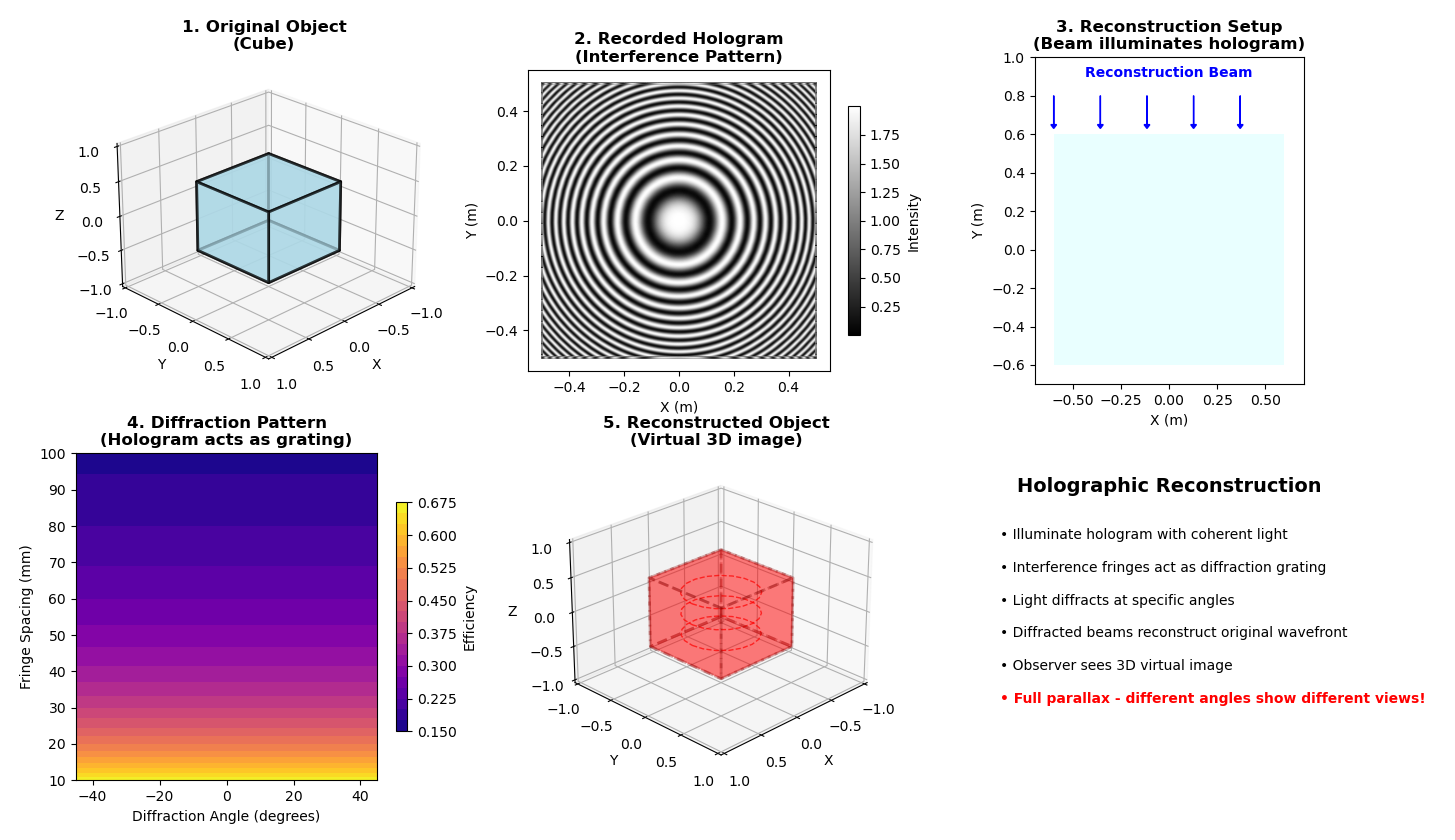
\includegraphics[width=0.9\textwidth]{Figures/cube-reconstruction.png}
        \caption{Reconstruction of the measured hologram of the 3D modelled cube.}
        \label{fig:cube_reconstruction}
    \end{figure}
\end{frame}
\begin{frame}{Holography: Reconstruction process}
    \begin{figure}[h]
        \centering
        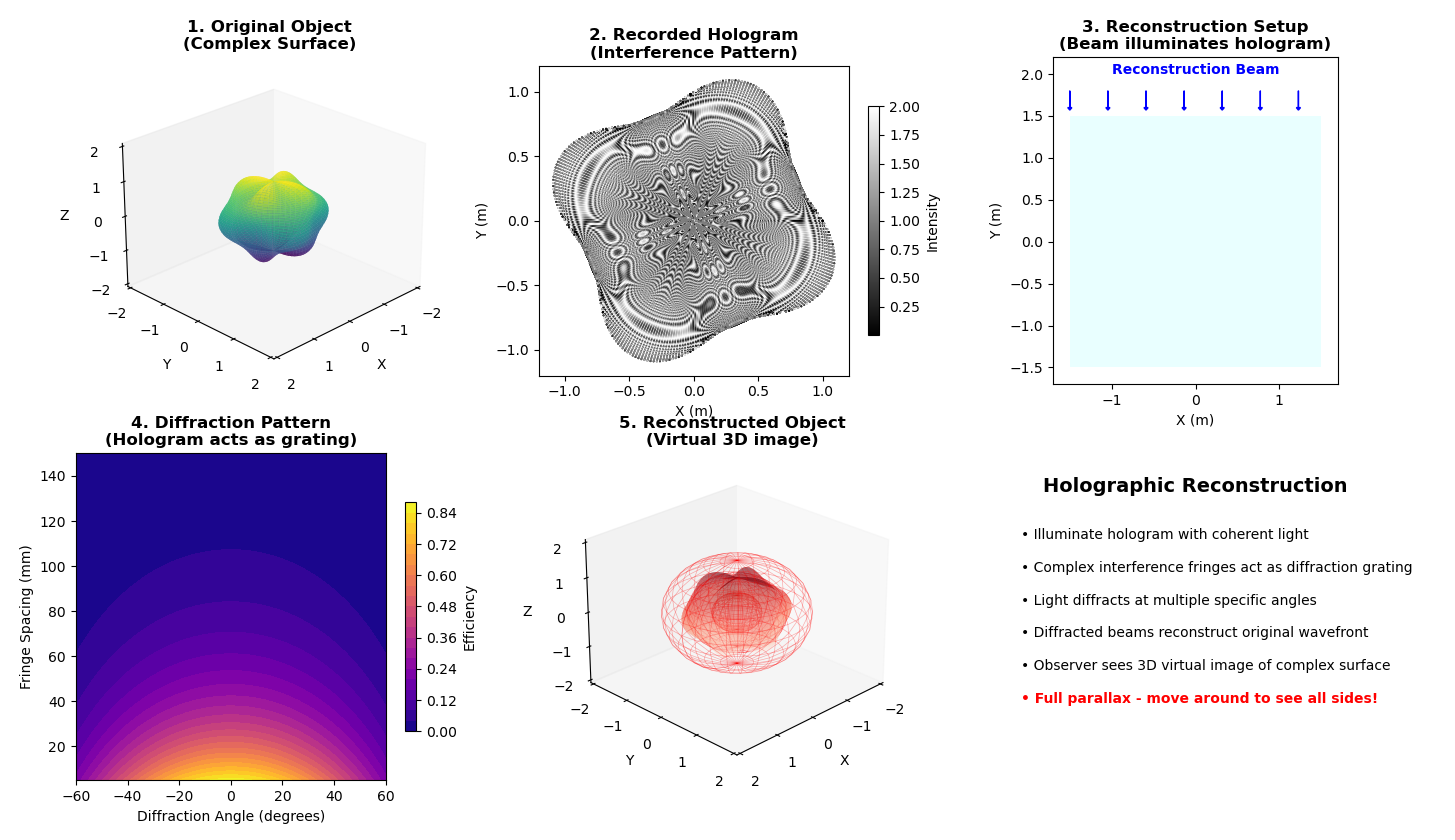
\includegraphics[width=0.9\textwidth]{Figures/sphere-reconstruction.png}
        \caption{Reconstruction of the measured hologram of the 3D modelled complex volume.}
        \label{fig:sphere_reconstruction}
    \end{figure}
\end{frame}
\begin{frame}{Holography vs Traditional photgraphy}
    \begin{columns}[T]
        \begin{column}{0.48\textwidth}
            \textbf{Traditional Photography:}
            \begin{itemize}
                \item Records only \textbf{2D intensity} information
                \item Single viewing perspective
                \item Loses all depth information
                \item Flat projection of 3D world
                \item Cannot reconstruct original light field
            \end{itemize}
        \end{column}
        \begin{column}{0.48\textwidth}
            \textbf{Holography:}
            \begin{itemize}
                \item Records \textbf{3D wavefront} information
                \item Multiple viewing perspectives encoded
                \item Preserves complete depth information
                \item \textbf{All visible surfaces} from recording direction
                \item Reconstructs original light field
            \end{itemize}
        \end{column}
    \end{columns}
\end{frame}
\begin{frame}{Holography vs Ray-Tracing}
    \begin{itemize}
        \item Holography captures 3D information \textbf{just like ray-tracing} - limited by optical visibility
        \item But uses \textbf{interferometry \& diffraction} instead of computational algorithms
        \item Each recorded interference pattern encodes distances to all visible surface points
        \item Reconstruction reverses the process using wave optics principles
    \end{itemize}
\end{frame}
\section{Physics of Holographic Interferometry}
\begin{frame}{Physics of Holographic Interferometry}
    Now we can combine the concepts and explore the underlying physics of this optical technique.
    \begin{itemize}
        \item Double-exposure method
        \item Real-time method
        \item Time-averaged method
        \item Fringe formation and interpretation
        \item Sensitivity and measurement capabilities
    \end{itemize}
\end{frame}
\begin{frame}{Double-exposure method}

\end{frame}
\begin{frame}{Real-time method}

\end{frame}
\begin{frame}{Time-averaged method}

\end{frame}
\begin{frame}{Fringe formation and interpretation}

\end{frame}
\begin{frame}{Sensitivity and measurement capabilities}

\end{frame}

\section{Industrial Applications}
\begin{frame}{Industrial Applications}
    This section will showcase the practical uses of holographic interferometry.
    \begin{itemize}
        \item Non-destructive testing (NDT)
        \item Stress and strain analysis
        \item Vibration analysis
        \item Flow visualization
        \item Surface contouring and deformation measurement
    \end{itemize}
\end{frame}
\begin{frame}{Industrial Applications: Non-destructive testing}

\end{frame}
\begin{frame}{Industrial Applications: Stress and strain analysis}

\end{frame}
\begin{frame}{Industrial Applications: Vibration analysis}

\end{frame}
\begin{frame}{Industrial Applications: Flow visualization}

\end{frame}
\begin{frame}{Industrial Applications: Surface and deformation measurement}

\end{frame}

\section{Conclusion}
\begin{frame}{Conclusion}
    A summary of the key concepts presented.
    \begin{itemize}
        \item Recap of holographic interferometry principles
        \item Advantages and limitations
        \item Future outlook and potential advancements
    \end{itemize}
\end{frame}

% Optional: Add a frame for references if you have a .bib file
% \section{References}
% \begin{frame}[allowframebreaks]{References}
%   \bibliographystyle{plain}
%   \bibliography{references} % Assuming you have a references.bib file
% \end{frame}

\end{document} 